\textbf{\textit{“Good architecture makes the system easy to understand, easy to develop, easy to maintain, and easy to deploy. The ultimate goal is to minimize the lifetime cost of the system and to maximize programmer productivity.” - Robert C. Martin}} \cite{10}

Software systems grow and change over the time. As a software system changes, the interactions between different system elements lead to complexity. To develop reliable software systems that can overcome this complexity, programmers must implement software systems in a generalized fashion. Software systems written in such a fashion can be considered reliably usable, maintainable, testable, and extendable \cite{15}. This fashion is called software architecture. Martin Fowler defines the software architecture as "the shared understanding that the expert developers have of the system design" \cite{16}. The formal definition of software architecture is "the set of significant decisions about the organization of a software system, the selection of structural elements and their interfaces by which the system is composed, together with their behaviour as specified in the collaborations among those elements, the composition of these elements into progressively larger subsystems, and the architectural style that guides this organization -- these elements and their interfaces, their collaborations, and their composition" \cite{17}. The role of software architecture in software development can be elaborated under the six major aspects. Those aspects can be listed as follows \cite{25}:
\begin{itemize}
    \item \textbf{Understanding:} Software architecture simplifies the understanding and improves the readability of software systems.
    \item \textbf{Reuse:} Software architecture facilitates  the code reuse between the components.
    \item \textbf{Construction:} Software describes the components of the system and dependencies between those components.
    \item \textbf{Evolution:} Software architecture helps developers to understand the consequences of changes more accurately and describes the concerns of the software systems.
    \item \textbf{Analysis:} Software architecture enables analyzing the system consistency, compliance with restrictions imposed by the architecture, and with the quality attributes.
    \item \textbf{Management:} Assessment of software architecture facilitates understanding of risks, requirements, and implementation strategies.
\end{itemize}

When the list above is examined, the effects of these roles on the maintainability of software systems are obvious. This situation is also clearly demonstrated in a related study. This study has researched Android practitioners, grey literature and white literature, analyzing many relevant resources regarding Android application architecture. Results of the study revealed that the top quality requirement for Android application architecture is maintainability \cite{14}.
\begin{figure}[ht!]
    \centering
    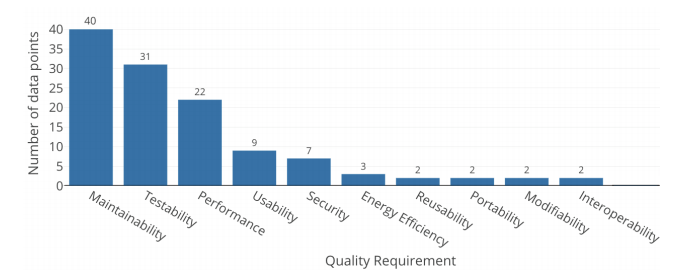
\includegraphics[scale=0.5]{figures/quality_req.png}
    \caption{Quality requirement rankings for Android app architecture \protect\cite{14}}
    \label{fig:arch_quality_req_ranking}
\end{figure}
\FloatBarrier

Also, other quality requirements presented in Fig. \ref{fig:arch_quality_req_ranking}, such as modifiability, reusability, and testability, correlate with maintainability  \cite{53}. Consequently, the impact of the architecture on the maintainability of software systems is one of the top aspects that should be considered before starting the development.

When architecting Android applications, several different architectural and design patterns are preferred by Android community. Verdecchia et al. (2019) present the developer tendencies in their study \cite{14}. However, considering that their study is from 2019 and the tendencies of Android developers change fast, there might be slight changes in these developer tendencies. Their work also predicted the possible changes.
\begin{figure}[ht!]
    \centering
    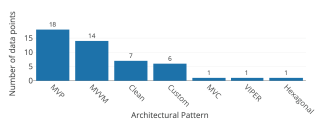
\includegraphics[scale=1]{figures/android-architecture.png}
    \caption{Developer tendencies for Android app architecture \protect\cite{14}}
    \label{fig:android-architecture}
\end{figure}
\FloatBarrier

Implementation and theoretical details of such architectural and design patterns are beyond the scope of this study. However, considering the importance of architectural and design pattern choice for the maintainability of Android applications, briefly explaining a few important ones is necessary. As shown in Fig. \ref{fig:android-architecture}, Model-View-Presenter (MVP), Model-View-View Model (MVVM), and Clean Architecture are the most popular ones. MVP and MVVM are two different derivatives of the MV+X model. They are widely used in GUI-heavy applications. These architectural patterns are built on top of SOLID and separation of concerns principles. They separate application into data, logic and view layers where every layer has its own responsibility \cite{48}. Robert C. Martin introduced Clean Architecture Principles in 2012 \cite{10}. In his book, he indicates that “The goal of software architecture is to minimize the human resources required to build and maintain the required system”. Clean Architecture consolidates software engineering practices to produce quality systems with some specifications such as maintainability, testability and so on. The most important characteristic of Clean Architecture is having independent layers. The idea is that nothing in an inward layer ought to rely upon anything in an external layer. Specifically, application and business rules should not rely upon UI, database, moderators, etc. These tenets enable us to create Android applications that are less complex to keep updated as changes in the external circles will not affect the inward ones \cite{58}.